\chapter{Results}
\section{Implementation of Randomness in the Logistic Map}
\section{Implementation of Randomness in the Circle Map}
\begin{figure}[!h]
\caption[Average number of order $p$ orbits for the random
circle map]{Average number of order $p$ periodic orbits for the random
circle map, where $L=0.1$, $\omega =0.1$ and $k=1$. Results from 1000
simulations of these parameters are plotted.}
	\begin{center}
		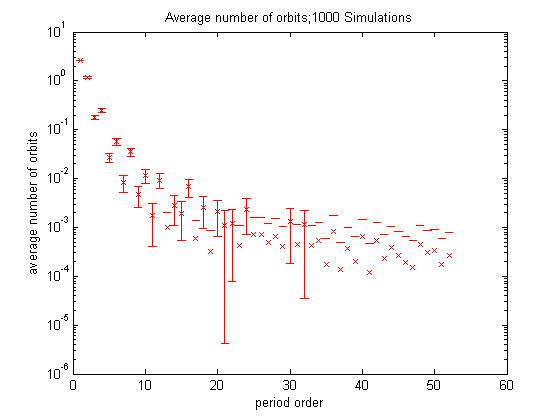
\includegraphics[scale=0.7]{figs/rcirc_avg_num_1000_sim_logscale.png}
	\end{center}
\end{figure}

\begin{figure}[!h]
\caption[Bifurcation diagram of the random
circle map]{Bifurcation diagram of the random
circle map for $L=0.1$, $\omega \in [0,1]$, $\Delta \omega = 0.001$
and $k=1$. Results from 100 simulations of these parameters are
plotted. Blue: period 1, red:
period 2, cyan: period 3, magenta: period 4, green: period 5, black:
period $p > 5$.} 
	\begin{center}
		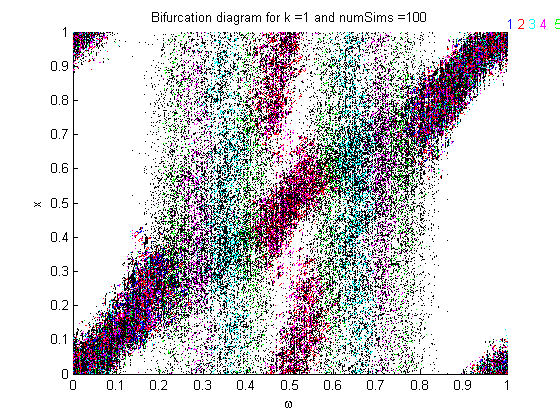
\includegraphics[scale=0.7]{figs/rcirc_bif_L01_k1.png}
	\end{center}
\end{figure}

\begin{figure}[htp]
\caption[The devil's staircase for the random circle map]{The devil's
  staircase for $k=1$ and $L = 0.1,0.5$. For small $L$
  (leftmost graph), the noise is more pronounced than for large $L$
  (rightmost graph).}\label{fig:randdevil1}
\centering
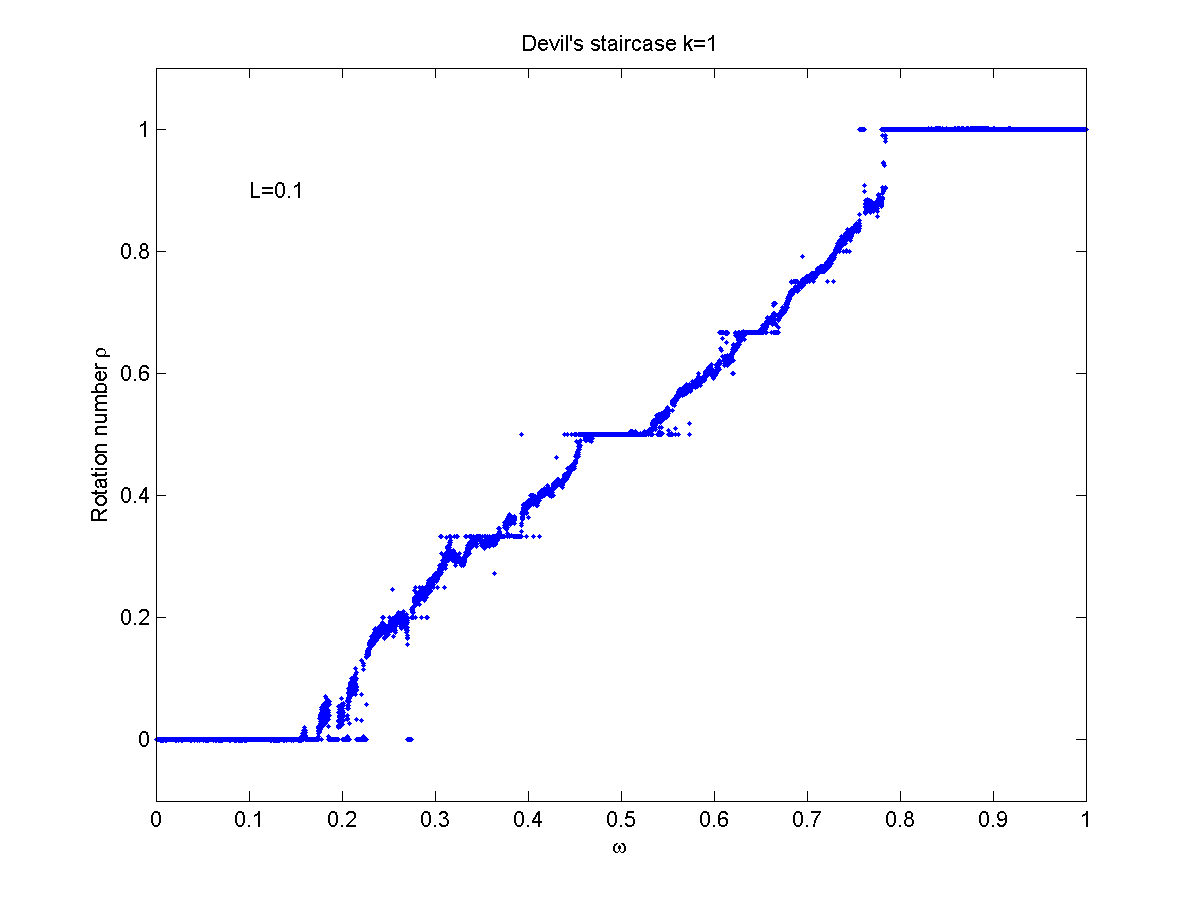
\includegraphics[width=.5\textwidth]{figs/rdevil_k1_L01.png}\hfill
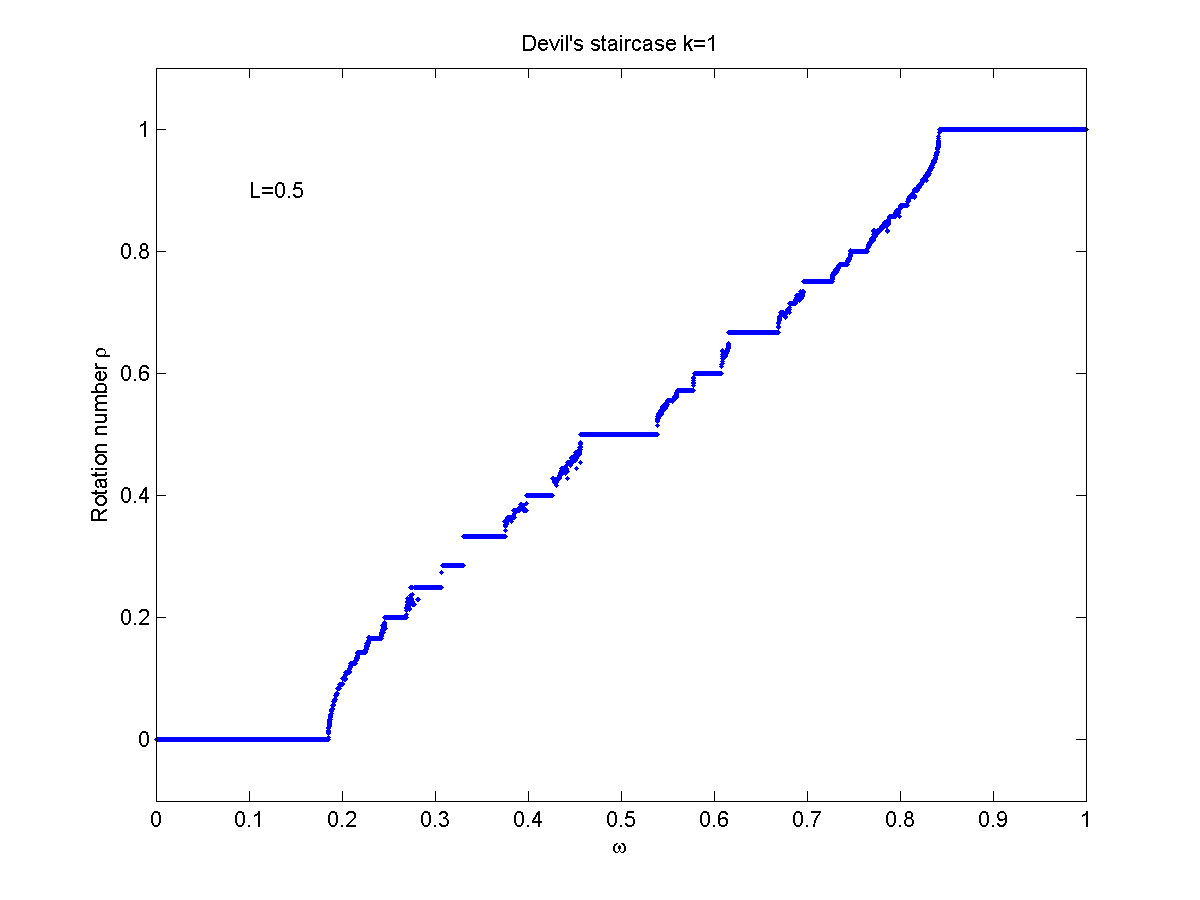
\includegraphics[width=.5\textwidth]{figs/rdevil_k1_L05.png}
\end{figure}

\begin{figure}[htp]
\caption[Histogram of rotation numbers in the random circle
map]{Histogram of rotation numbers in the random circle map, where
  $L=0.1$, $k=1$, and $\omega = 0.45$. Results from 1000 simulations
  are plotted.}
\centering
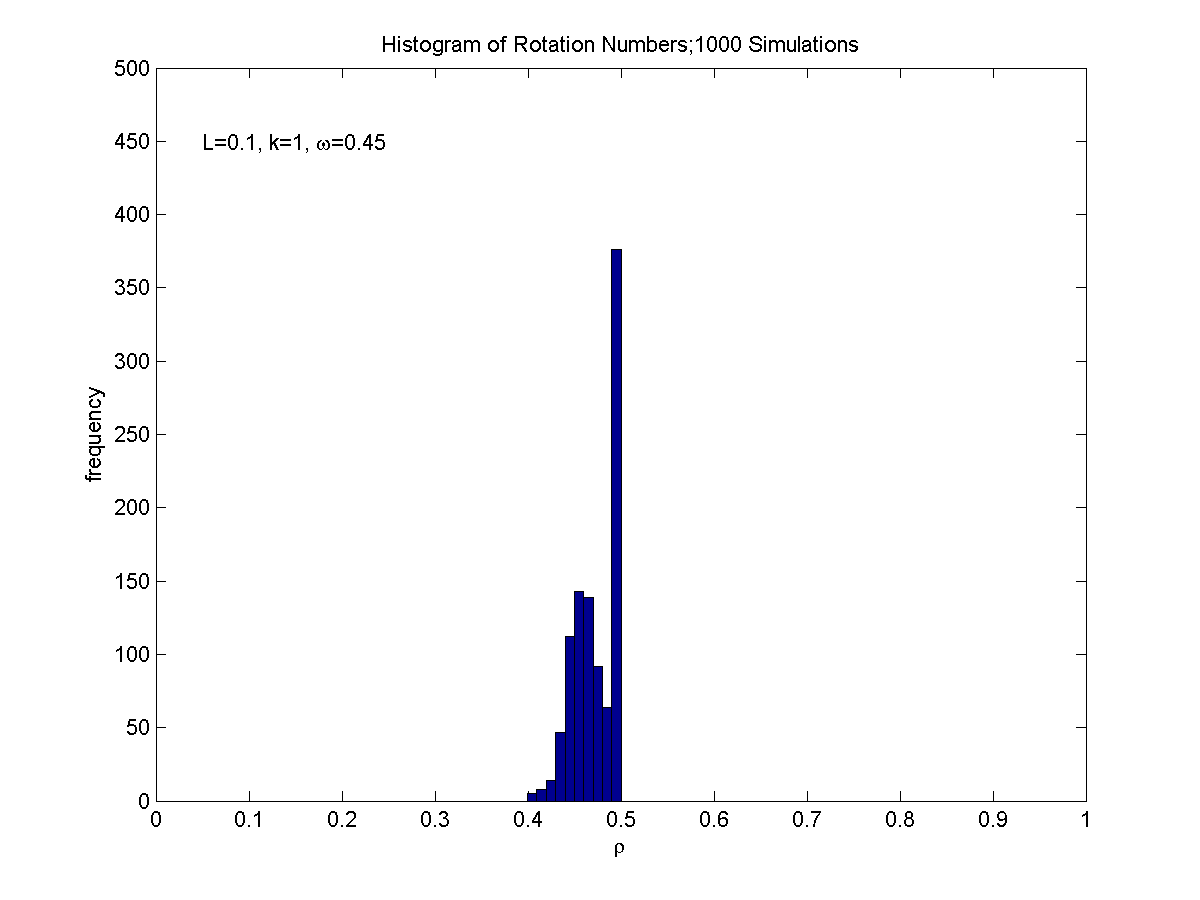
\includegraphics[width=.5\textwidth]{figs/hist_rho_k1_L01_om045.png}\hfill
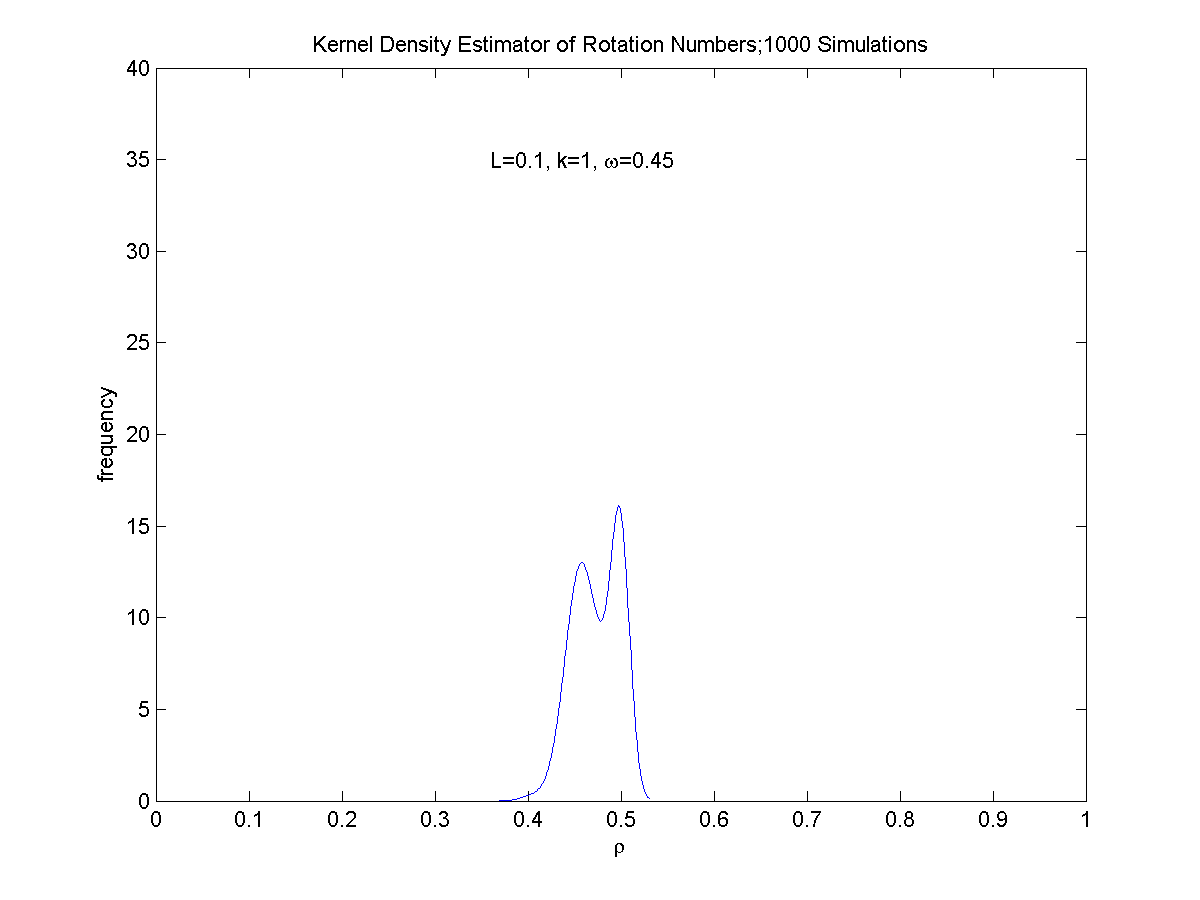
\includegraphics[width=.5\textwidth]{figs/kde_rho_k1_L01_om045.png}
\end{figure}

\begin{figure}[htp]
\caption[The Arnold tongues for the random circle map]{The Arnold
  tongues for $k\in [0,1]$, $\Delta k = 0.001$, $\omega \in [0,1]$,
  $\Delta \omega = 0.001$ and $L_j =0.1j$, where $j = 1, 2, 3, 4, 7,
  9$. Plots are ordered left to right, and top to bottom. Red: period 1
  fixed points, black: orbits that have period larger than 100 (or
  possibly no period), orange: period 2 orbit, yellow: period 3 orbit, blue: period 5 orbit,
green: period 4 orbit, and purple: period 6 orbit.}\label{fig:randtongues}
\centering
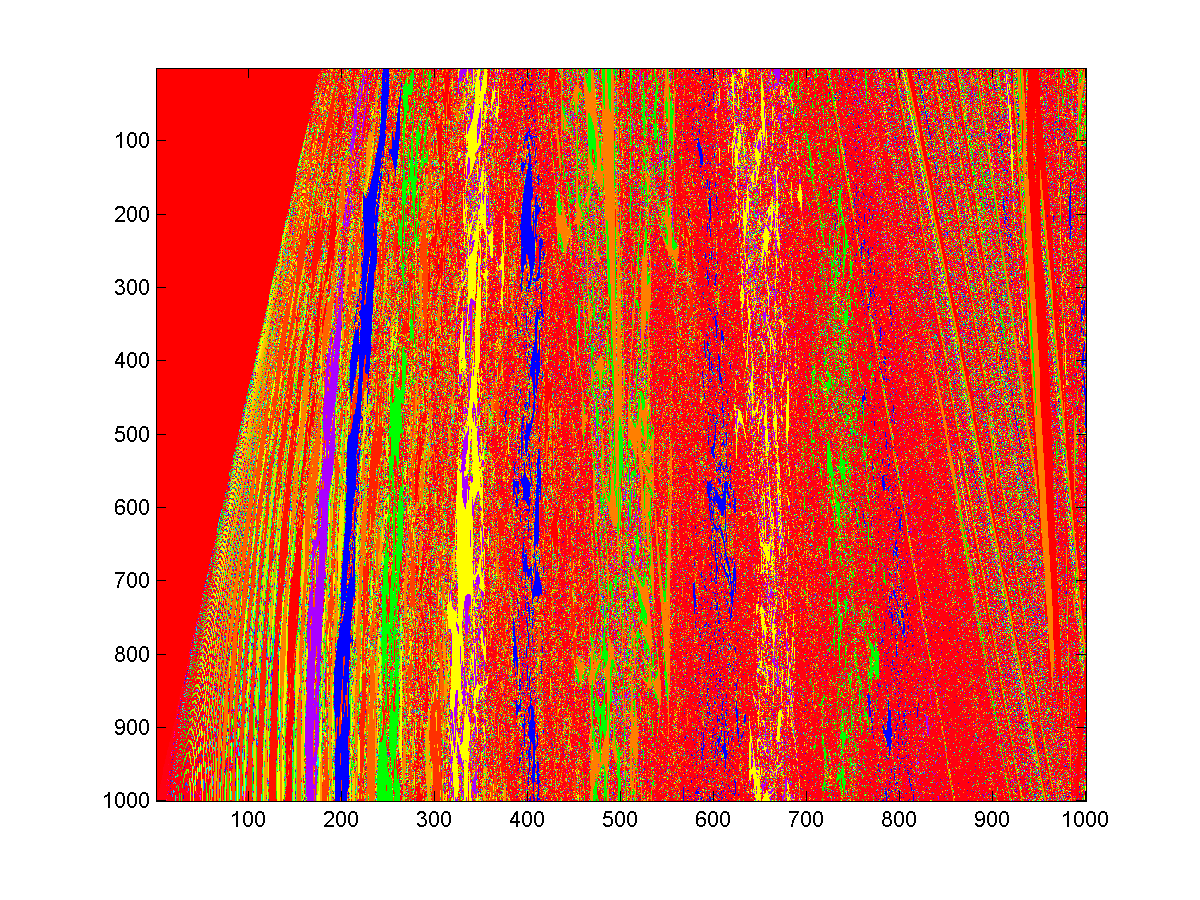
\includegraphics[width=.5\textwidth]{figs/tongues_1000_L_01.png}\hfill
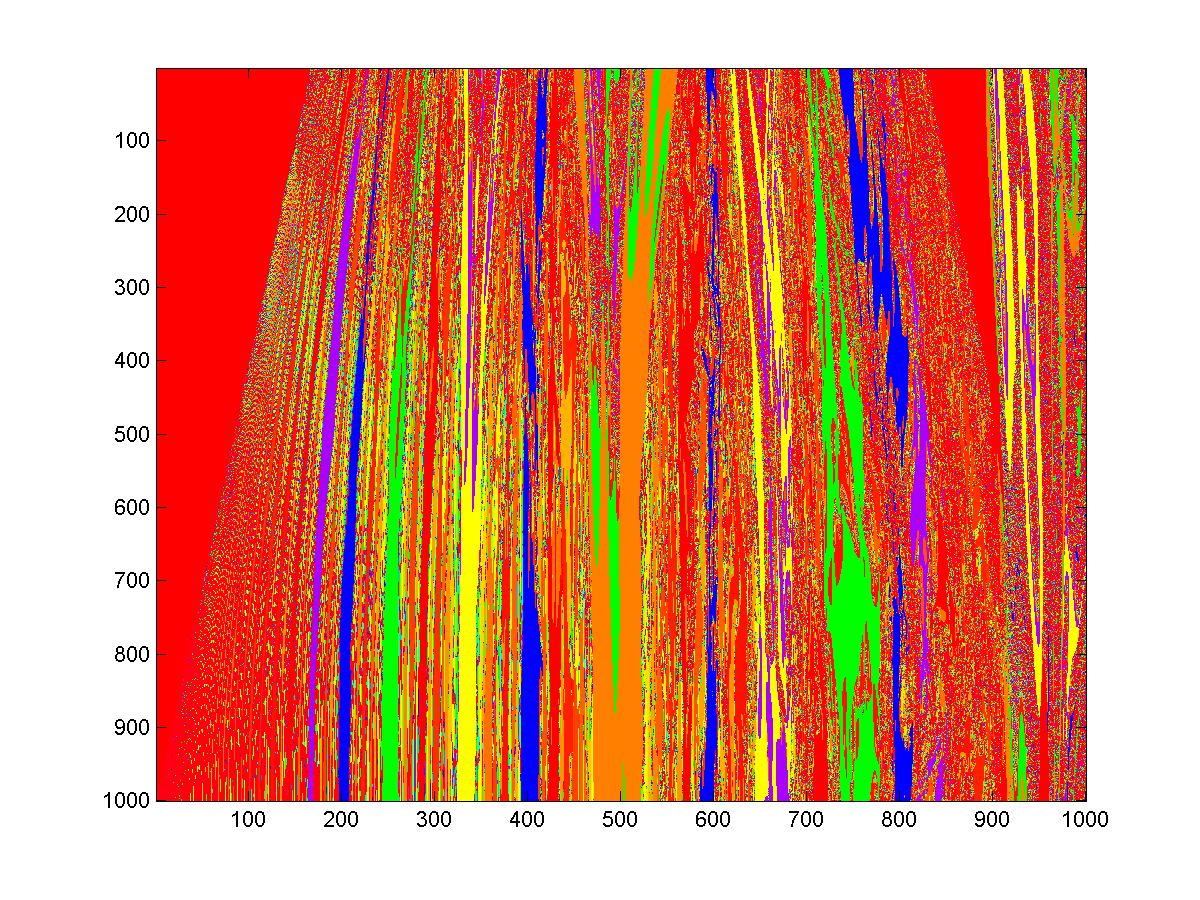
\includegraphics[width=.5\textwidth]{figs/tongues_1000_L_02.png}\\
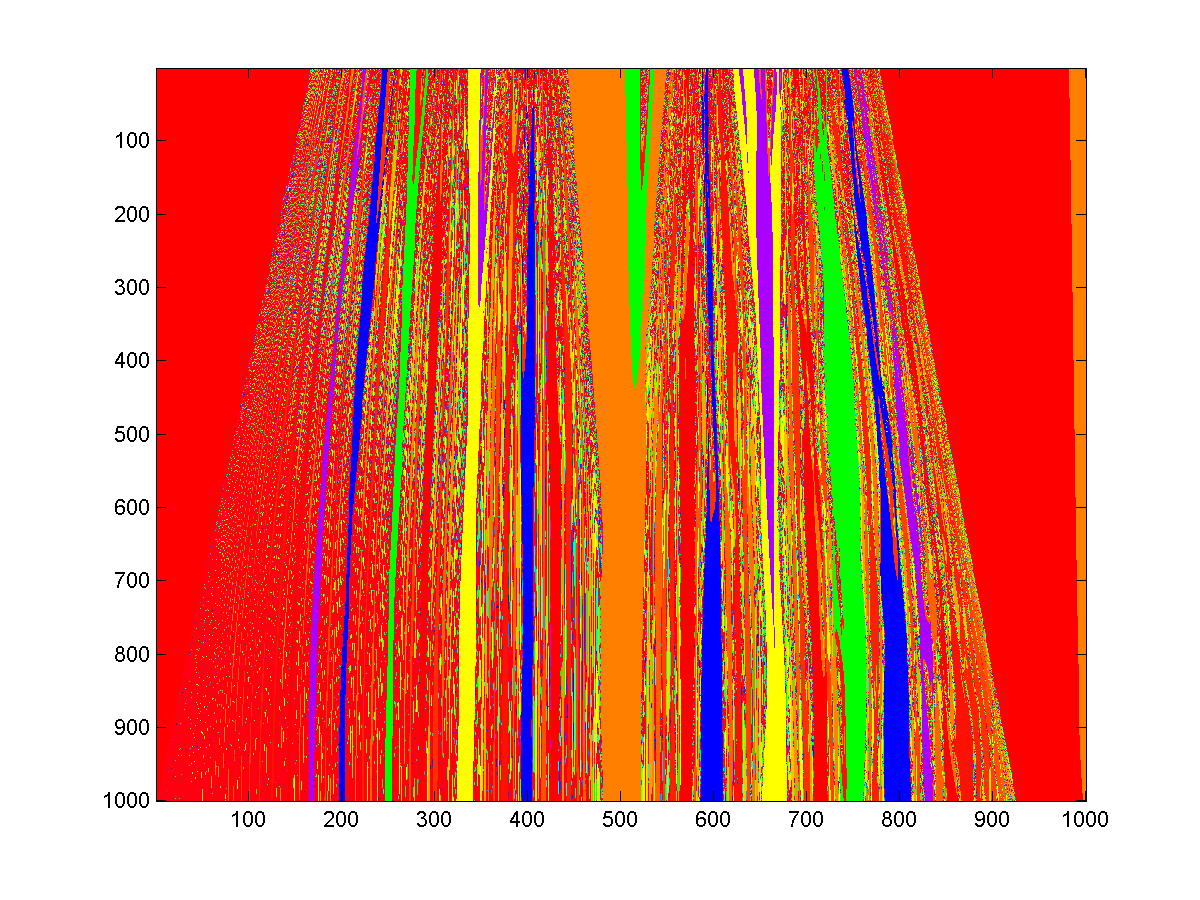
\includegraphics[width=.5\textwidth]{figs/tongues_1000_L_03.png}\hfill
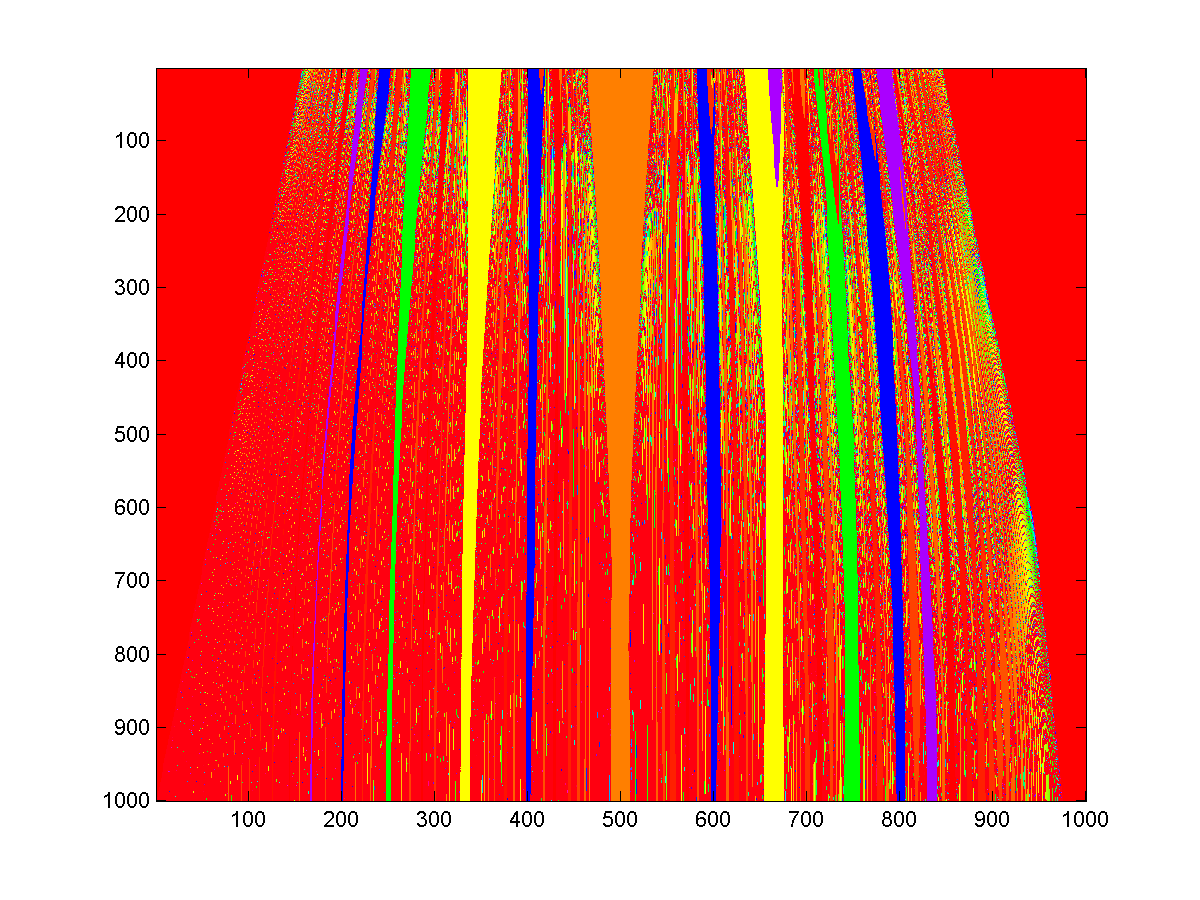
\includegraphics[width=.5\textwidth]{figs/tongues_1000_L_04.png}\\
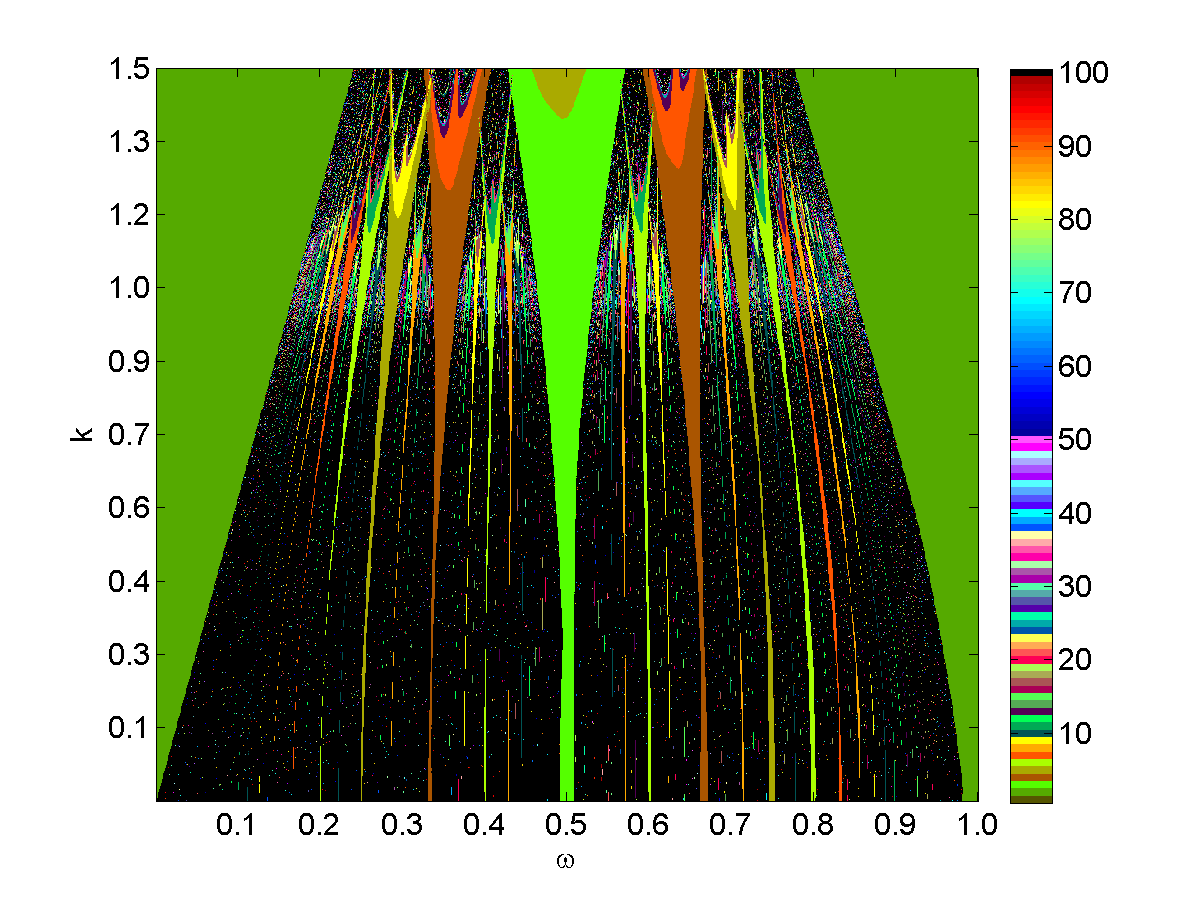
\includegraphics[width=.5\textwidth]{figs/tongues_1000_L_07.png}\hfill
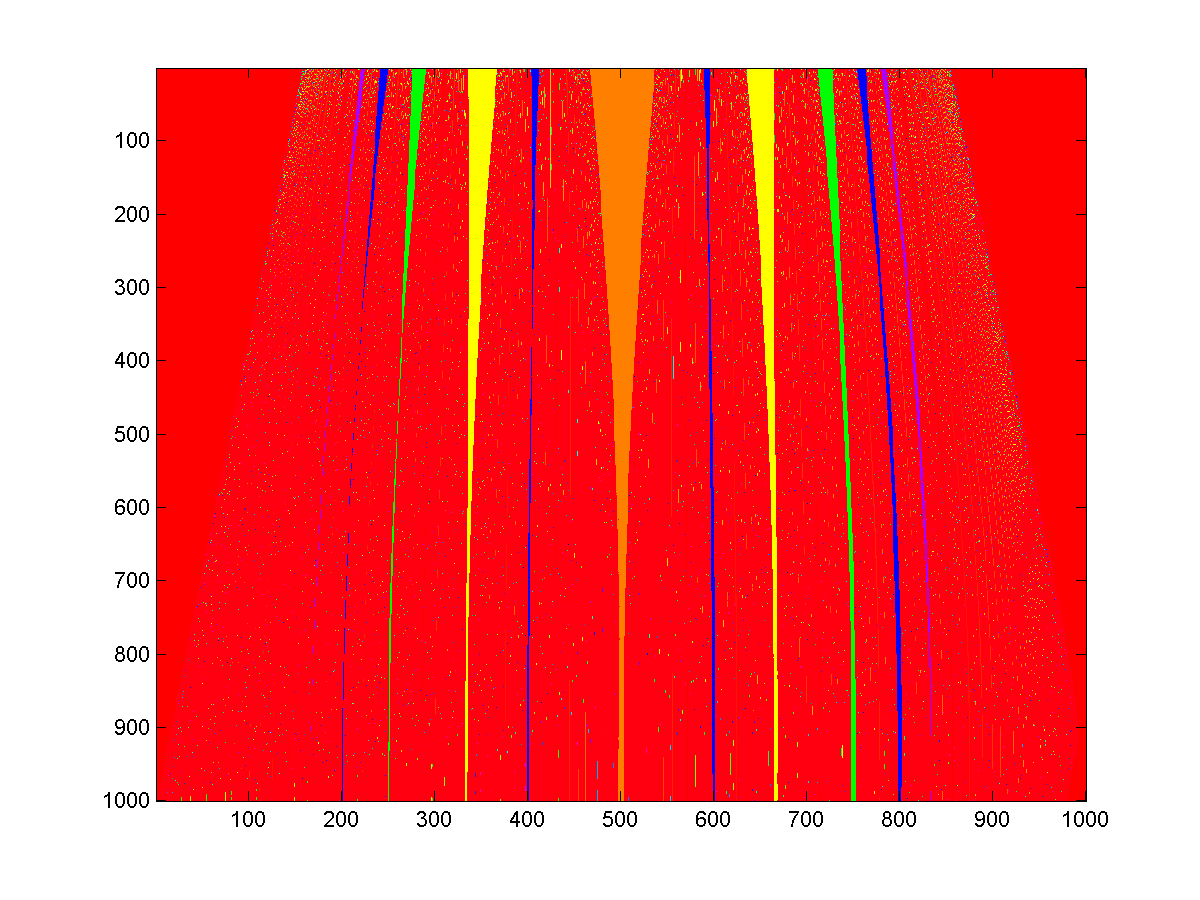
\includegraphics[width=.5\textwidth]{figs/tongues_1000_L_09.png}\\
\end{figure}


